\documentclass[12pt,letterpaper,english,bibliography=totocnumbered, abstract=on]{scrartcl}

\usepackage{indentfirst}
\usepackage[titletoc]{appendix}
\usepackage[T1]{fontenc}
\usepackage[latin9]{inputenc}
\usepackage{color}
\usepackage{babel}
\usepackage{verbatim}
\usepackage[unicode=true,pdfusetitle,
bookmarks=true,bookmarksnumbered=false,bookmarksopen=false,
breaklinks=true,pdfborder={0 0 0},pdfborderstyle={},backref=false,colorlinks=true]
{hyperref}
\hypersetup{linkcolor=blue,citecolor=blue,urlcolor=blue}

\usepackage{booktabs}
\usepackage{multirow}
\usepackage{adjustbox}
\usepackage{threeparttable}
\usepackage[table]{xcolor}
\usepackage{csquotes}
\usepackage{soul} % for hiliting text: \hl

\usepackage[backend=biber, style=authoryear, maxbibnames=99, dashed=false]{biblatex}
\setlength\bibitemsep{2\itemsep}
\addbibresource{../CRB.bib}

\usepackage{pdfpages}
\usepackage{float} % Allows use of H to place floats

\usepackage{pgfgantt}

\usepackage{framed}

\usepackage{datetime2}

\usepackage{courier}
\usepackage{listings}
\lstset{basicstyle=\tiny\ttfamily,
	columns=fullflexible,
	%basewidth=0.51em,
	frame=single}

% Prevent page breaks within paragraphs
% https://tex.stackexchange.com/questions/21983/how-to-avoid-page-breaks-inside-paragraphs
\widowpenalties 1 10000

\begin{document}

\titlehead{TECHNICAL REPORT}

\title{Development of Automated Roadside Video Surveys for Detecting and Monitoring Coconut Rhinoceros Beetle Damage}

%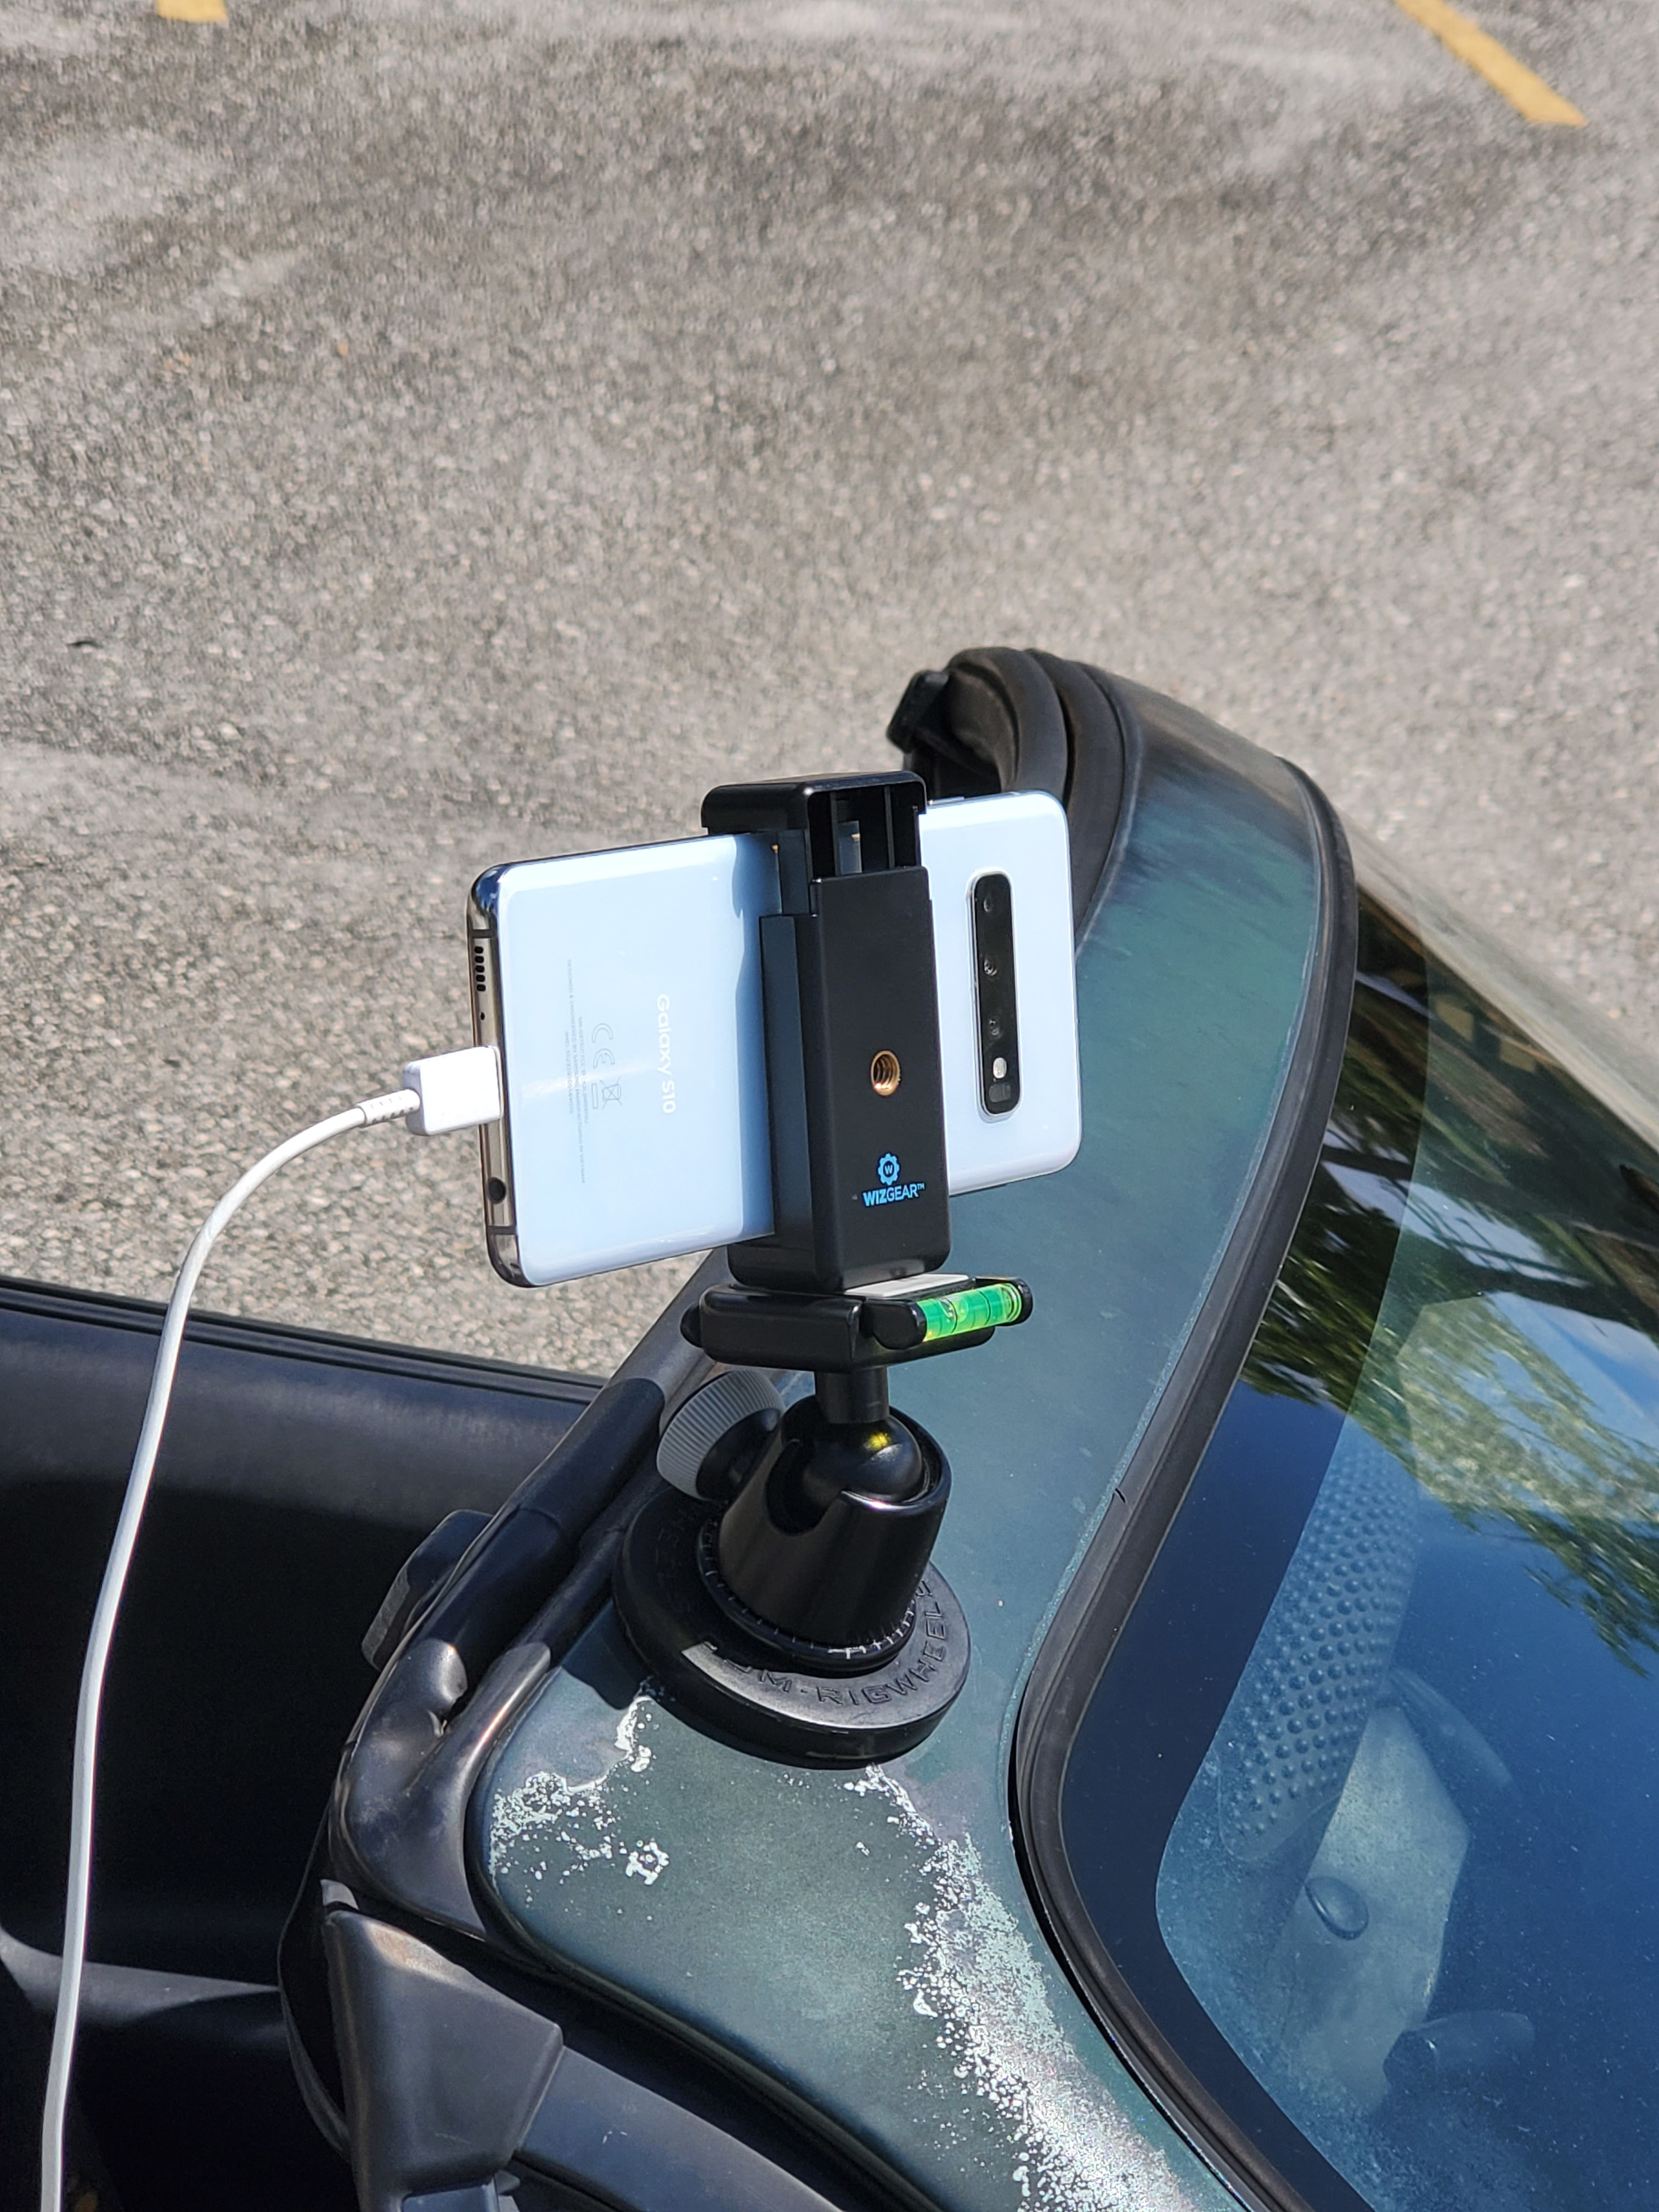
\includegraphics[width=0.25\textwidth]{images/car}
%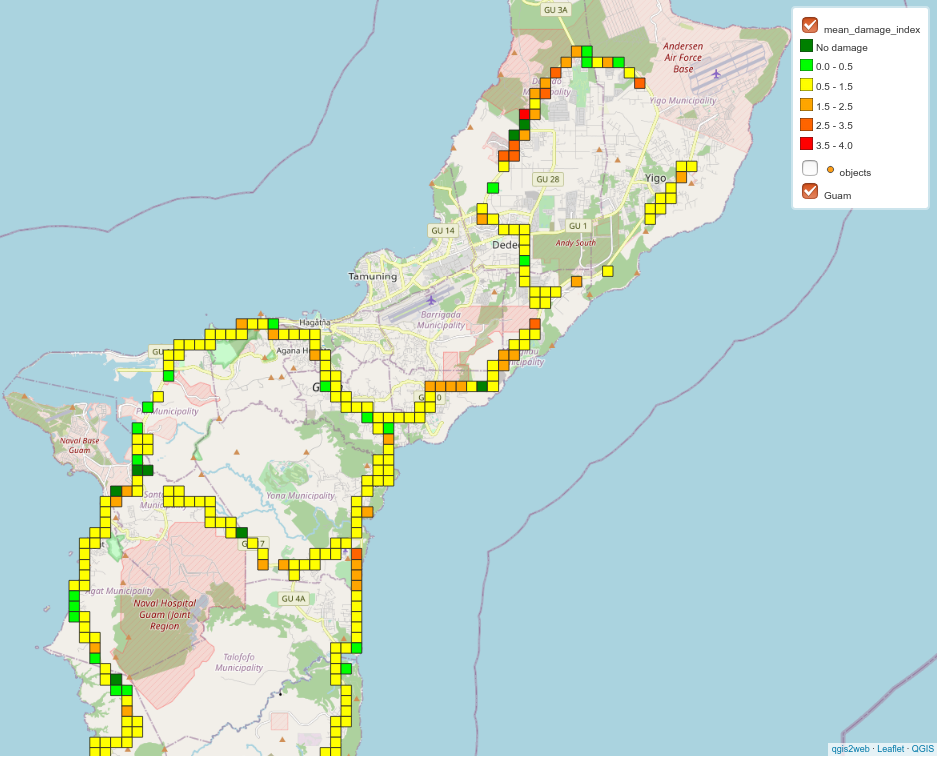
\includegraphics[width=0.7\textwidth]{images/webmap}

\author{Aubrey Moore}

\maketitle

\footnote{The most recent version of this document can be downloaded from\\
	\url{https://github.com/aubreymoore/roadside/blob/master/docs/roadside/roadside.pdf}.}

\newpage
\tableofcontents
\newpage
\lstlistoflistings
\newpage
\listoffigures
\newpage

\section{Background}

To see how coconut rhinoceros beetle damage surveys are currently done, please read \cite{jackson_rhinoceros_2019-1} and \cite{vaqalo_coconut_2017}.

\section{Recording Roadside Videos}

\subsection{Mounting a Smart Phone on a Vehicle}

Preliminary work show that mounting the smart phone externally produces much better results than mounting the phone internally as a dash cam. This eliminates problems cause by dirty windshields and internal reflections.  

A smart phone can be mounted externally using a ball and socket anchored using a strong magnet (\ref{fig:mount}).

Optimal placement of the smart phone camera appears to be above the right-hand corner of the windshield (passenger side in the US). 


\begin{figure}[H]
	\centering
	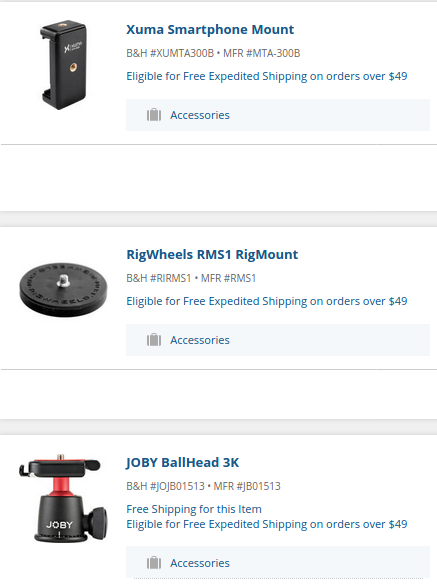
\includegraphics[width=0.7\linewidth]{images/mount}
	\caption{Smart phone mount.}
	\label{fig:mount}
\end{figure}

\subsubsection{Setting the Direction of View Angle}

The direction of view angle has two components, a horizontal angle with respect to direction of travel and a vertical angle. The horizontal angle is set using the scale at the base of the ball joint. The vertical angle is set using a free Android app called Clinometer (\url{https://play.google.com/store/apps/details?id=net.androgames.clinometer}) (Fig. \ref{fig:clinometer}).  

Optimal angles for direction of view appear to be 45 degrees to the right of direction off travel and 15 degrees above horizontal.

\begin{figure}[H]
	\centering
	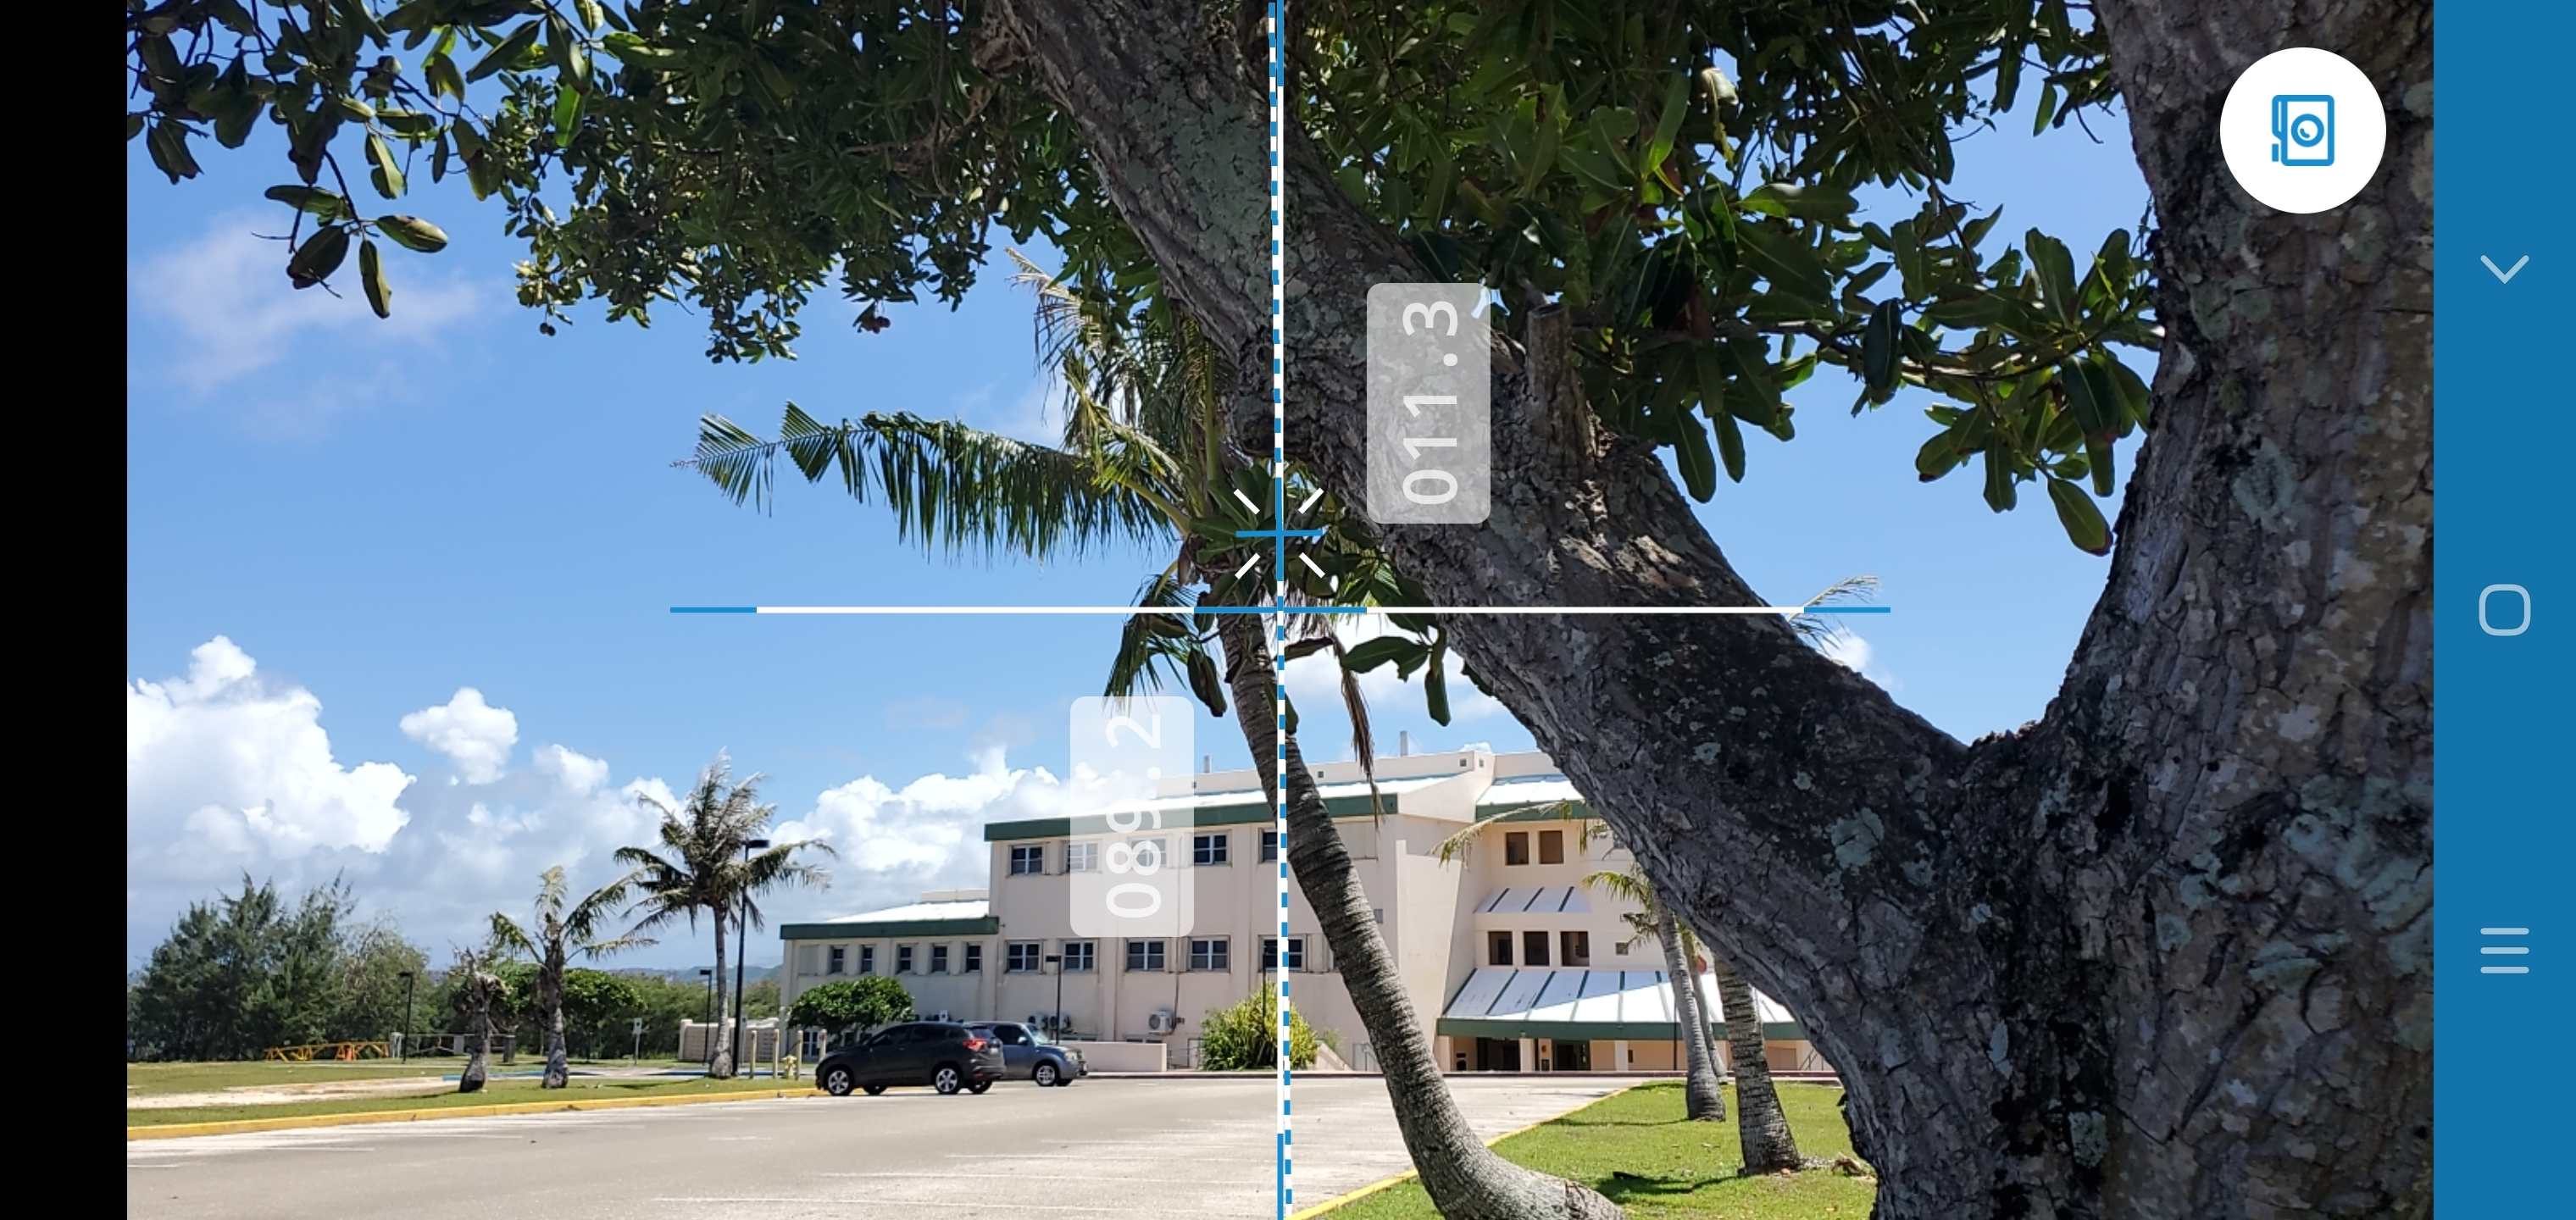
\includegraphics[width=0.7\linewidth]{images/clinometer}
	\caption{Setting camera angles using Clinometer app.}
	\label{fig:clinometer}
\end{figure}


\subsection{Parameter Choices}

\subsubsection{Camera and Lens}

We are currently using a Samsung Galaxy S10 smart phone.  This phone is equipped with four cameras including a 16MP ultra-wide-angle camera (123\textdegree{} field of view) which seems to be a good  choice for this application.

\subsubsection{Resolution}

Maximum resolution for videos recorded with the ultrawide angle camera is 4K 3840x2160 (16:9, 8.29MP). Initial recordings were made using this resolution, but this can probably be reduced without significant loss of precision.

\subsubsection{Frames per Second}

Standard frame rate is 30 fps. Initial recordings were made using this rate, but this can probably be reduced without significant loss of precision.

\subsection{Using the Open Camera App}

\textbf{Open Camera} (\url{https://opencamera.org.uk/}) is a FOSS app for Android smart phones which enables much better control of hardware features than the default Camera app provided with Samsung phones. 

\textbf{Open Camera} offers a plethora of settings which can be saved in a configuration file for later use. 
For screenshots of \textit{Video settings} see figures \ref{fig:videosettings1}, \ref{fig:videosettings2}, and \ref{fig:videosettings3}. 


\begin{figure}[H]
\centering
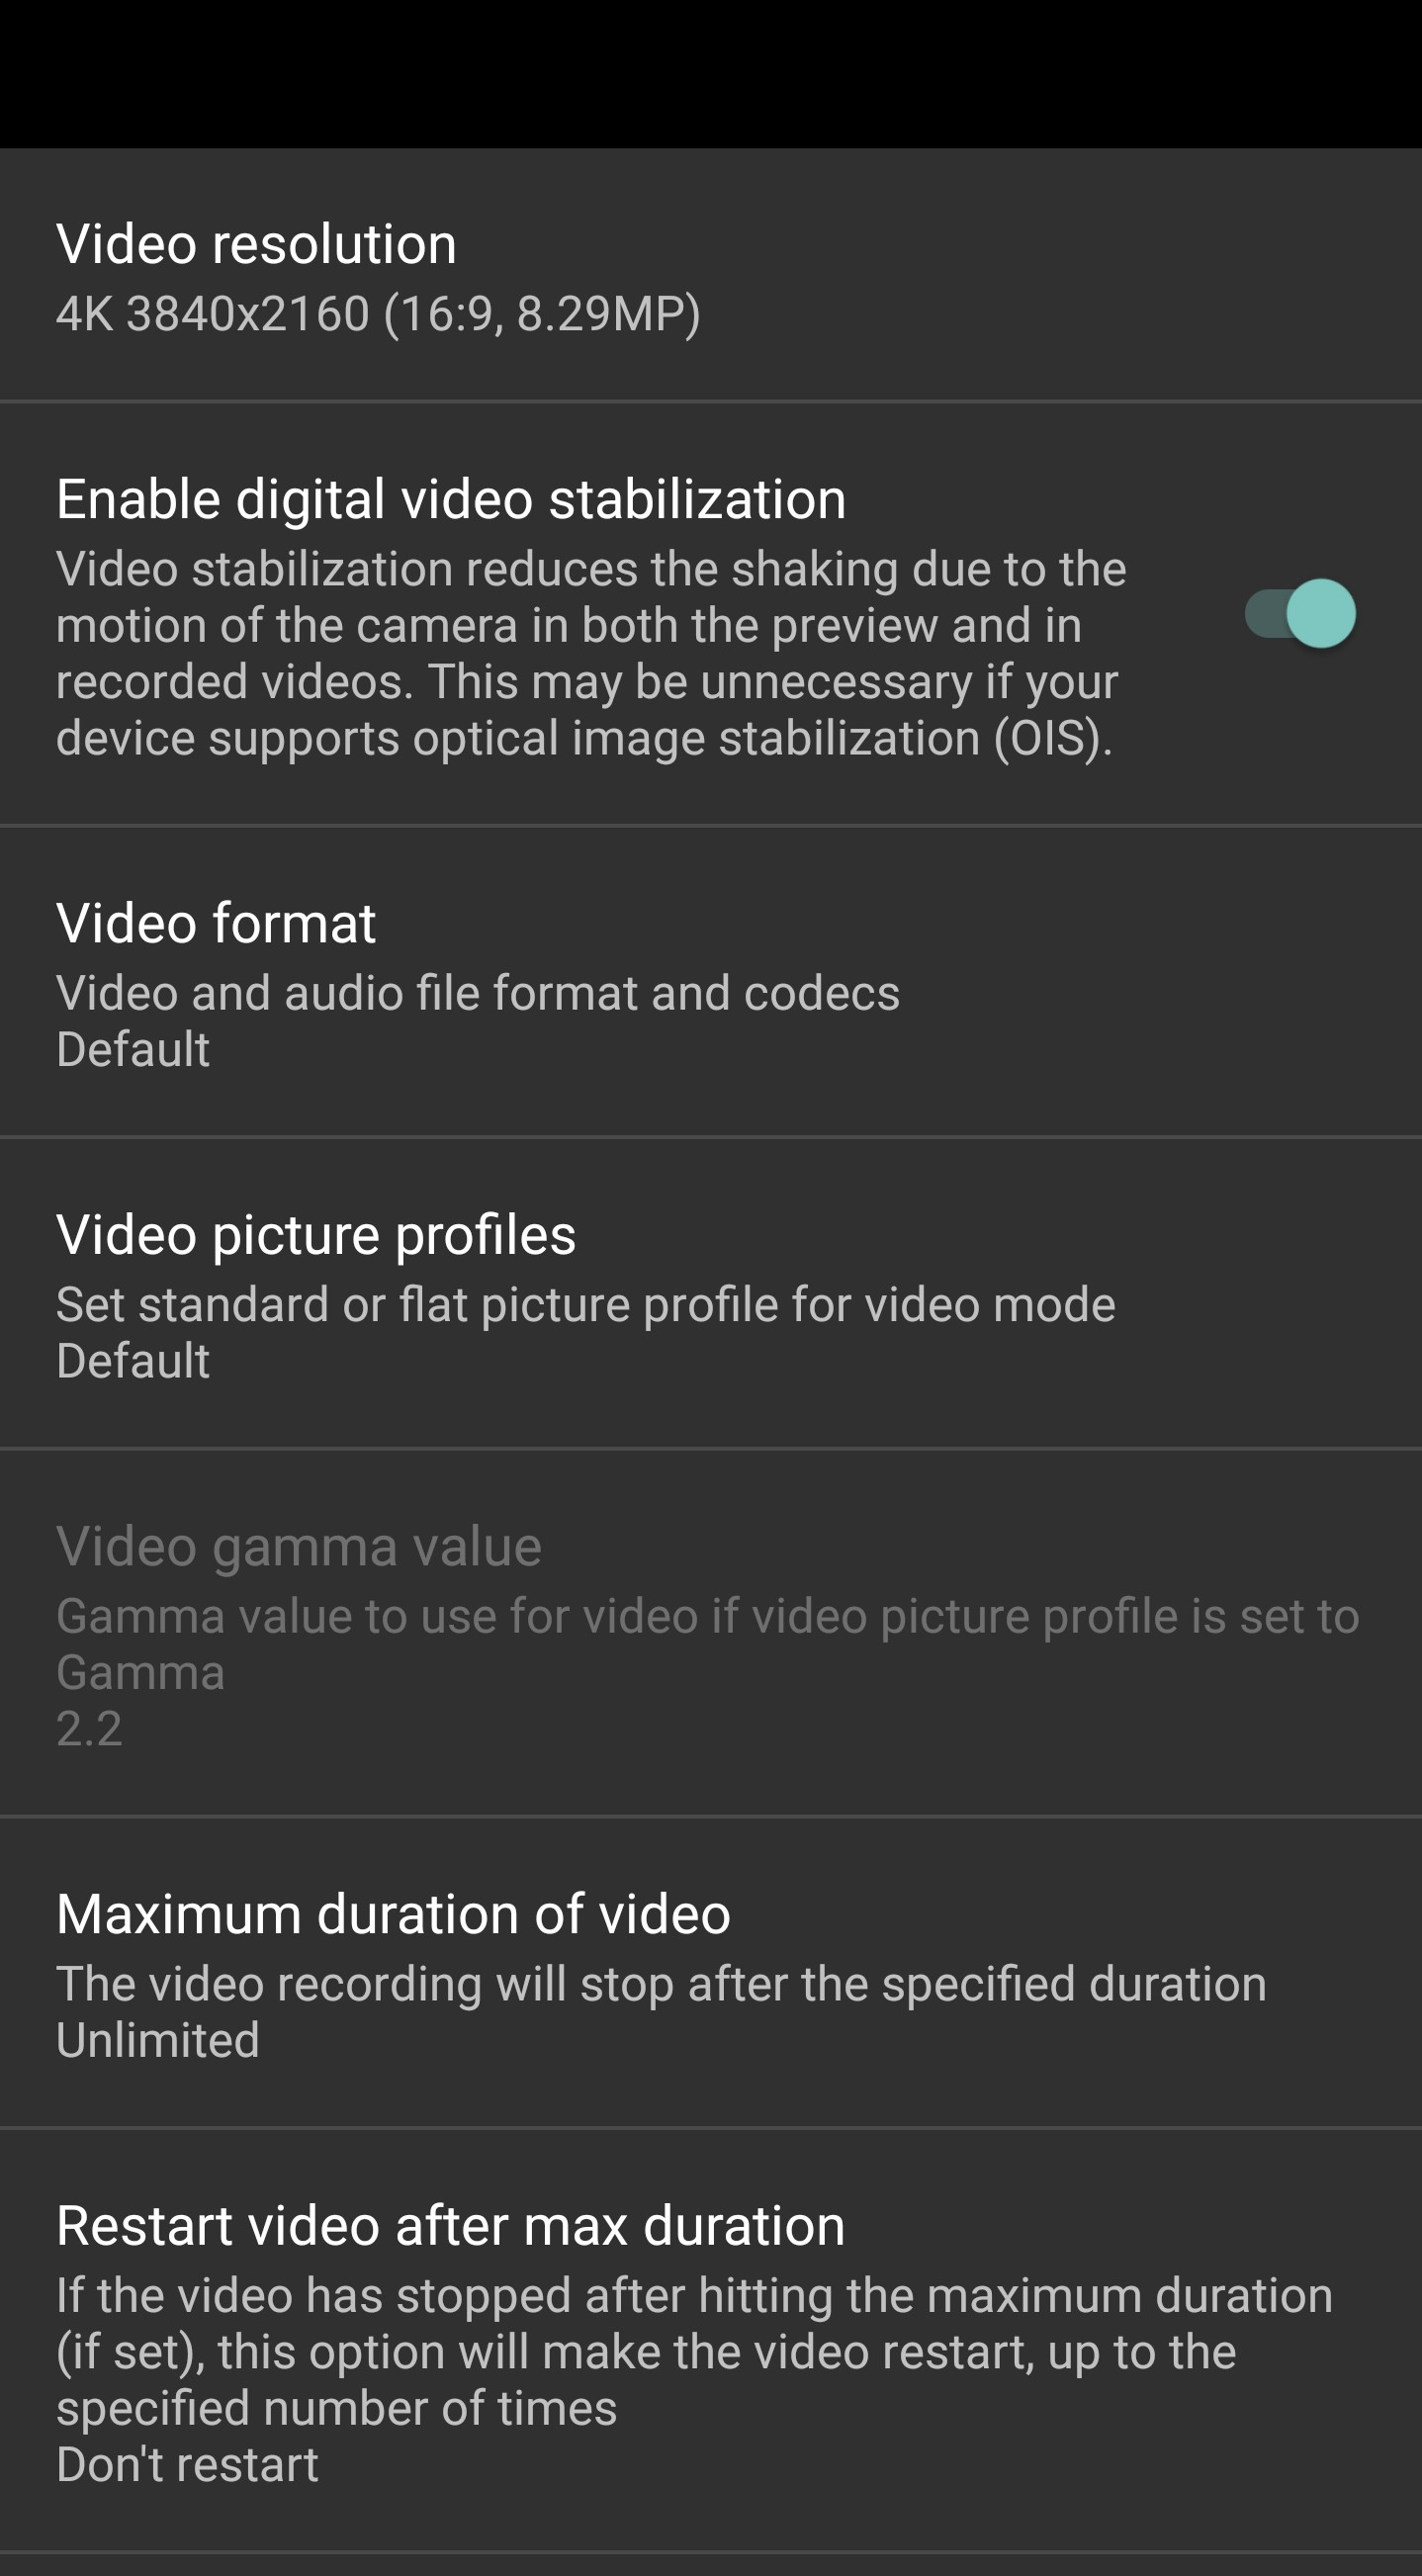
\includegraphics[width=0.7\linewidth]{images/videosettings1}
\caption{Video settings (1/3).}
\label{fig:videosettings1}
\end{figure}

\begin{figure}[H]
	\centering
	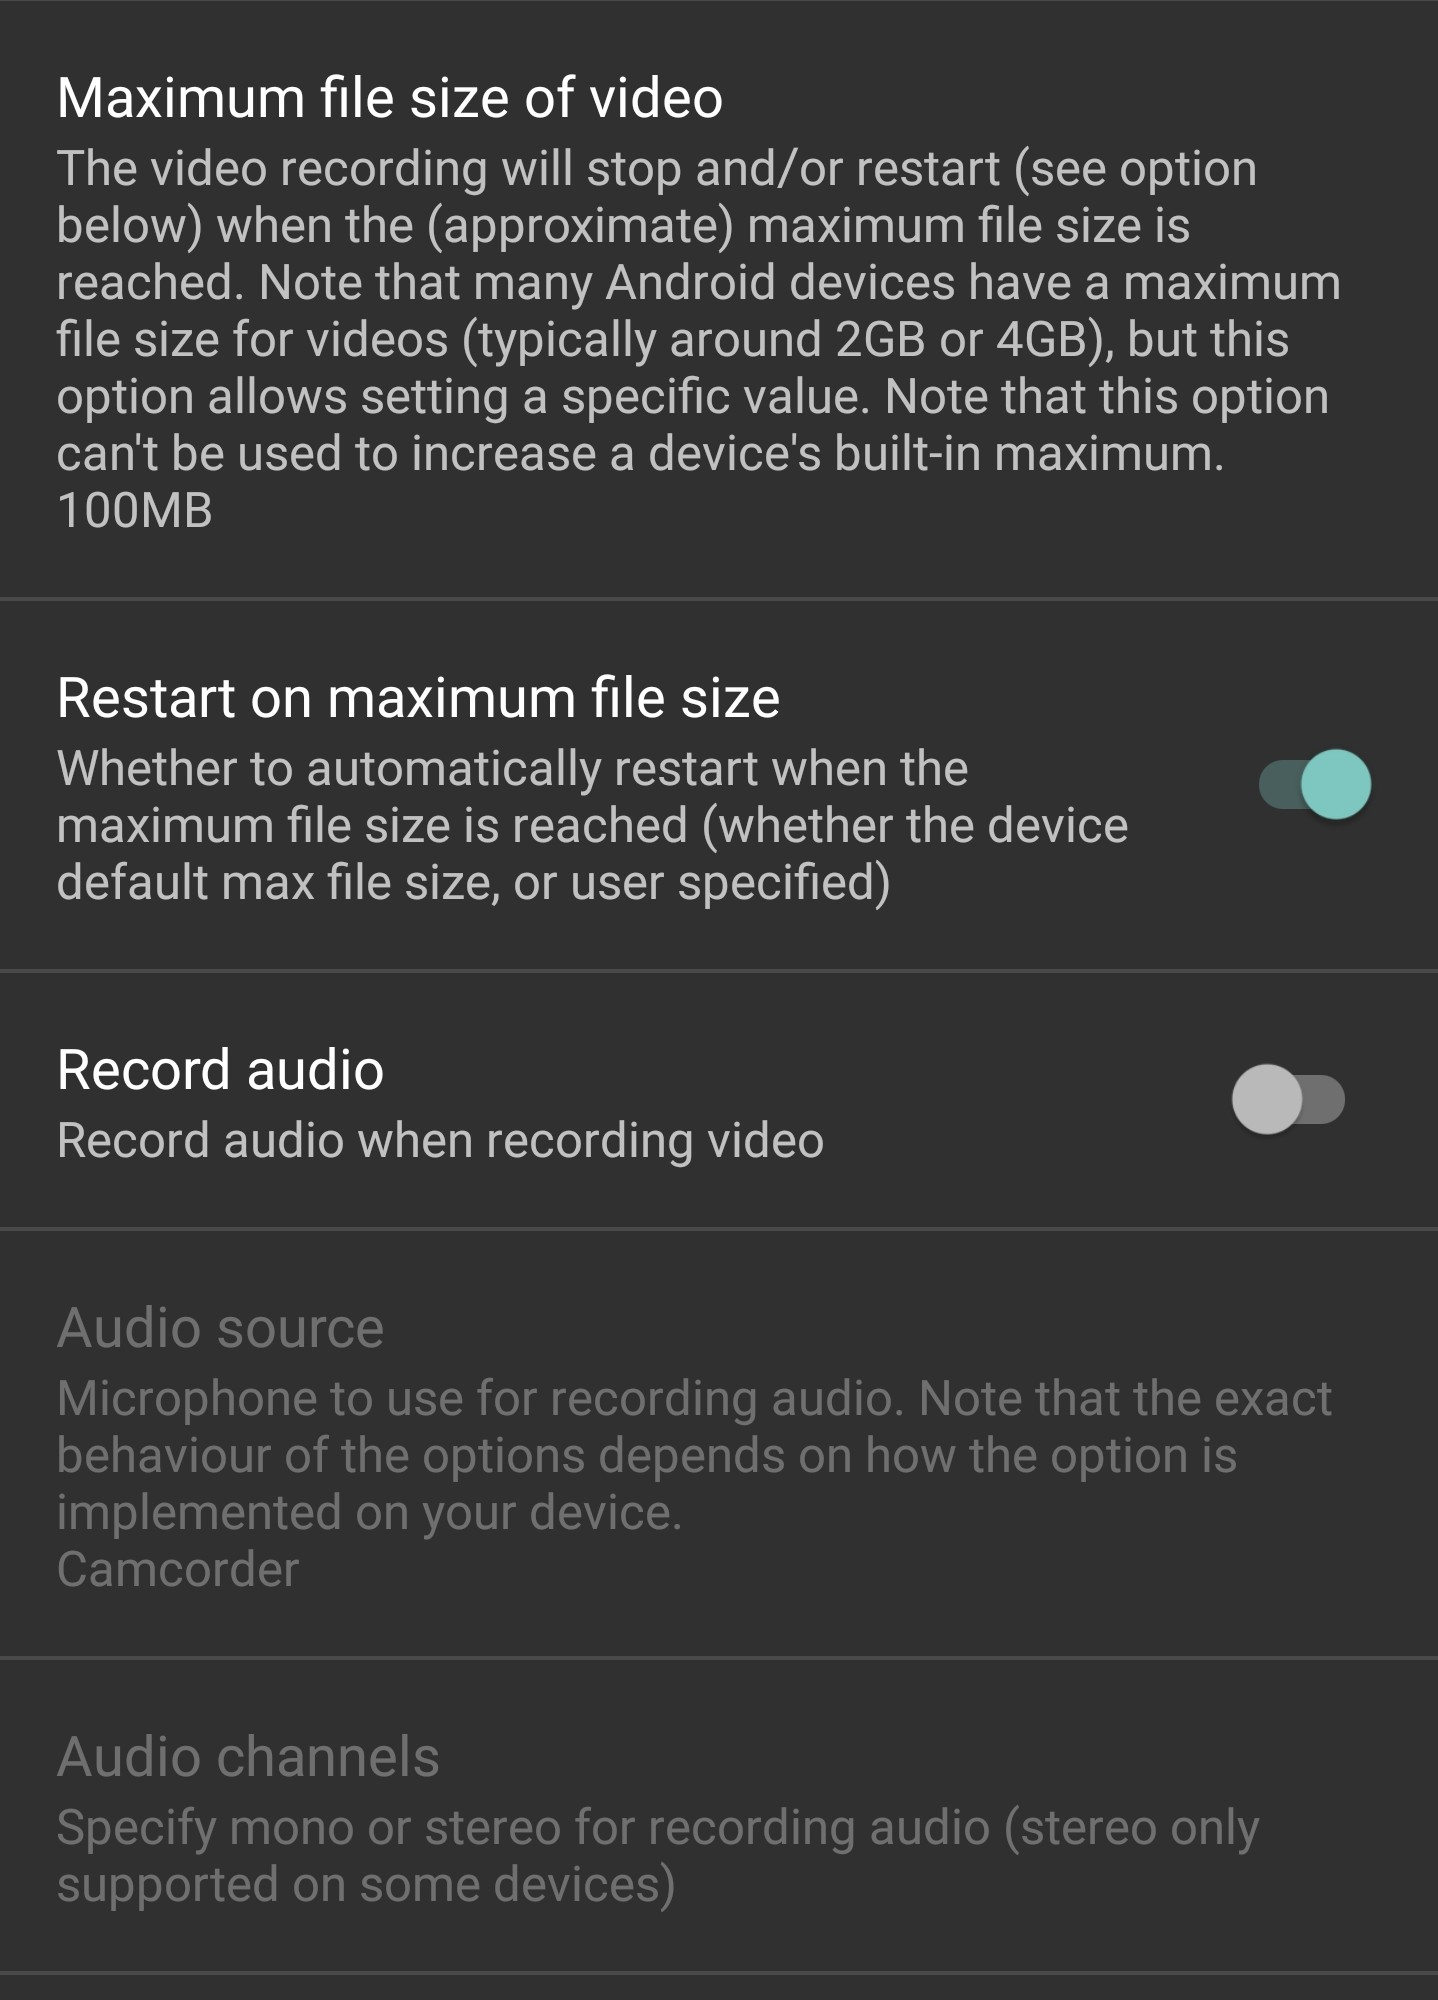
\includegraphics[width=0.7\linewidth]{images/videosettings2}
	\caption{Video settings (2/3).}
	\label{fig:videosettings2}
\end{figure}

\begin{figure}[H]
	\centering
	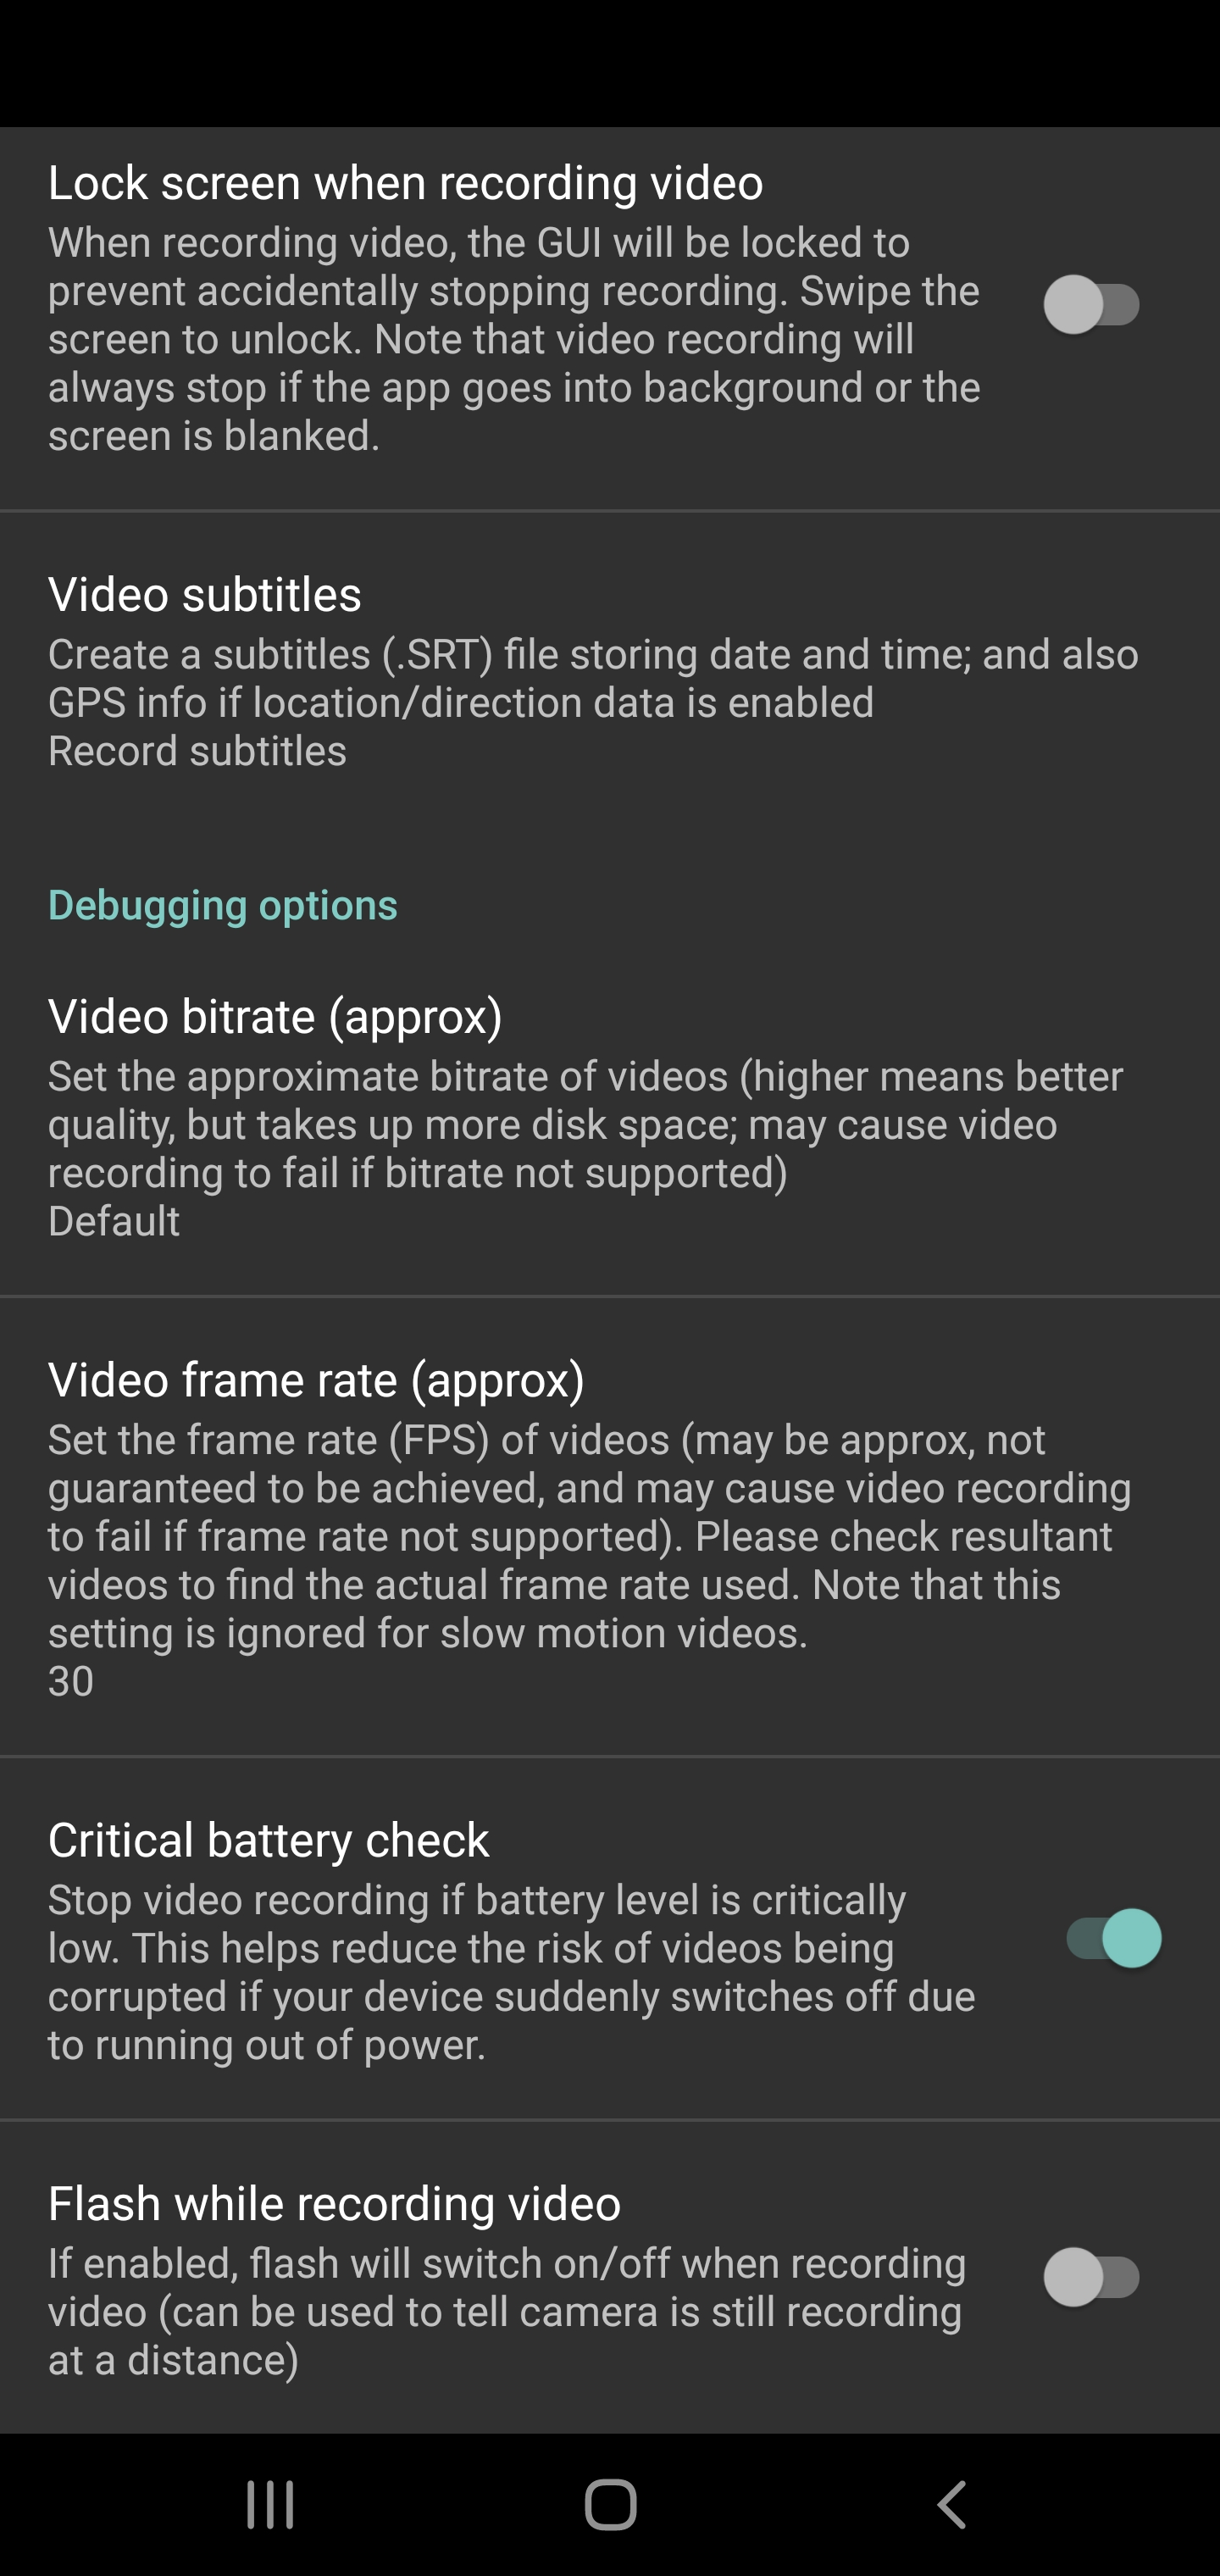
\includegraphics[width=0.7\linewidth]{images/videosettings3}
	\caption{Video settings (3/3).}
	\label{fig:videosettings3}
\end{figure}

\subsection{Using the GPSLogger App}

Although \textbf{Open Camera} has an option to georeference video frames, this feature proved unreliable in preliminary tests. As an alternative, it was decided to use a free called \textbf{GPSLogger} which logs timestamped GPS coordinates to a file at a frequency of once per second. \textbf{GPSLogger} runs continually in background on the phone during a series of video recordings.


\section{Data processing}

Data processing is controlled by a python script, process-data.py (Listing \ref{lst:process-data.py}).

\lstinputlisting[
language=python,
caption={process-data.py},
label={lst:process-data.py}
]{../../code/process-data.py}


\subsection{Georeferencing Video Frames}

The author has cobbled together a \textbf{jupyter notebook} called \textbf{georef} which uses the \textbf{GPSLogger} log to calculate the GPS coordinates for frames video recordings based on timestamps (seeinteractive map for displaying coconut rhinoceros beetle roadside video survey routes with popup thumbnail images at points of interest. The prototype map is at https://aubreymoore.github.io/qgiswebmap/webmap/webmap. )\url{https://github.com/aubreymoore/roadside/blob/master/jupyter%20notebooks/georef.ipynb}). 
	
\subsection{Mapping}

Interactive web maps for displaying coconut rhinoceros beetle roadside video survey routes with popup thumbnail images at points of interest can be put together using QGIS with the QGIS2WEB plugin. A prototype QGIS project is available in a GitHub repo at \url{https://github.com/aubreymoore/qgiswebmap} and a prototype map is available at \url{http://github.io/aubreymoore/qgiswebmap/webmap/webmap}.

\section{Detecting CRB Damage in Video Frames}

\section{Creating a CRB Damage Survey Database}

Have a look at database diagram (Fig. \ref{fig:erd}) and code listings \ref{createtables},  \ref{createviews} and \ref{creategrid}.

\begin{figure}[H]
	\centering
	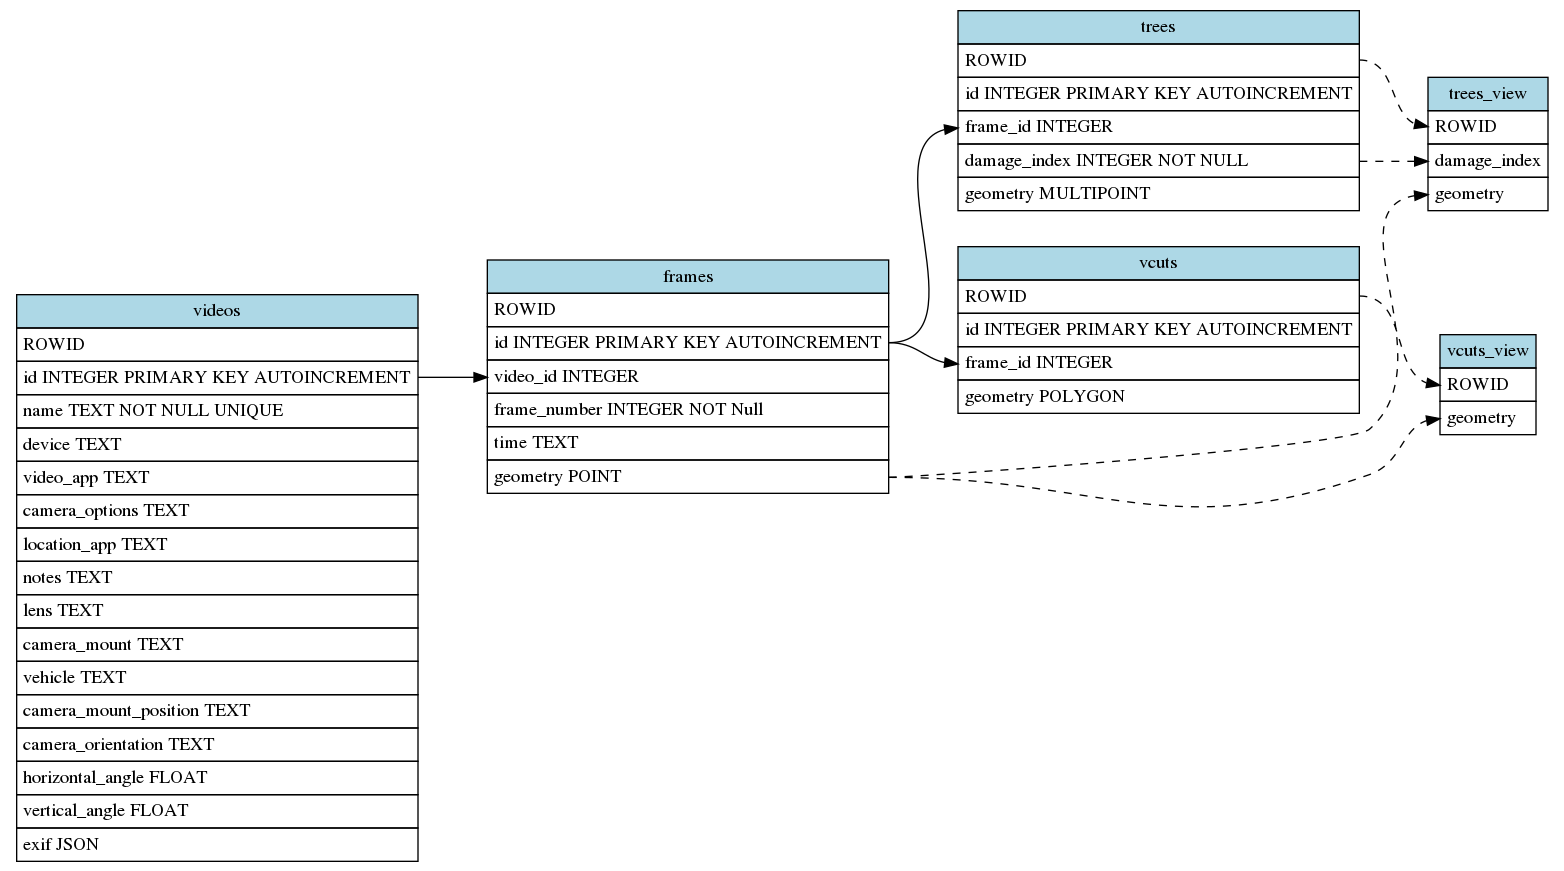
\includegraphics[width=\linewidth]{images/erd.png}
	\caption{Database diagram.}
	\label{fig:erd}
\end{figure}


\lstinputlisting[
language=SQL,
caption={create\_tables.sql},
label={createtables}
]{../../spatialite/create_tables.sql}


\lstinputlisting[
language=SQL, 
caption={create\_views.sql},
%float,
label={createviews}
]{../../spatialite/create_views.sql}

\lstinputlisting[
language=SQL, 
caption={create\_grid.sql},
label={creategrid}
]{../../spatialite/create_grid.sql}


\section{Visualizing Survey Results on a Map}

QGIS 3.16 was used to visualize survey results on a map. 

\begin{itemize}
	\item The map was made using a python script, 
	\textbf{create\_crb\_damage\_map.py}, 
	(Listing \ref{lst:create-crb-damage-map.py}) which reads data from 
	the spatialite database.
	\item An interactive web map is then created using the \textbf{qgis2web} plugin. 
	See Figures \ref{fig:qgis2web1} and \ref{fig:qgis2web2} for \textbf{qgis2web} parameters.
	\item The resulting	web map, stored in index.html, modified using edit\_webmap.py ().
	\item Finally, index.html was saved in
	a GitHub repository and published using GitHub pages.
\end{itemize}

\lstinputlisting[
language=python,
caption={make-crb-damage-map.py},
label={lst:make-crb-damage-map.py}
]{../../code/make-crb-damage-map.py}

%\lstinputlisting[
%language=python,
%caption={edit-webmap.py},
%label={lst:edit-webmap-data.py}
%]{../../code/edit-webmap.py}

\begin{figure}[H]
	\centering
	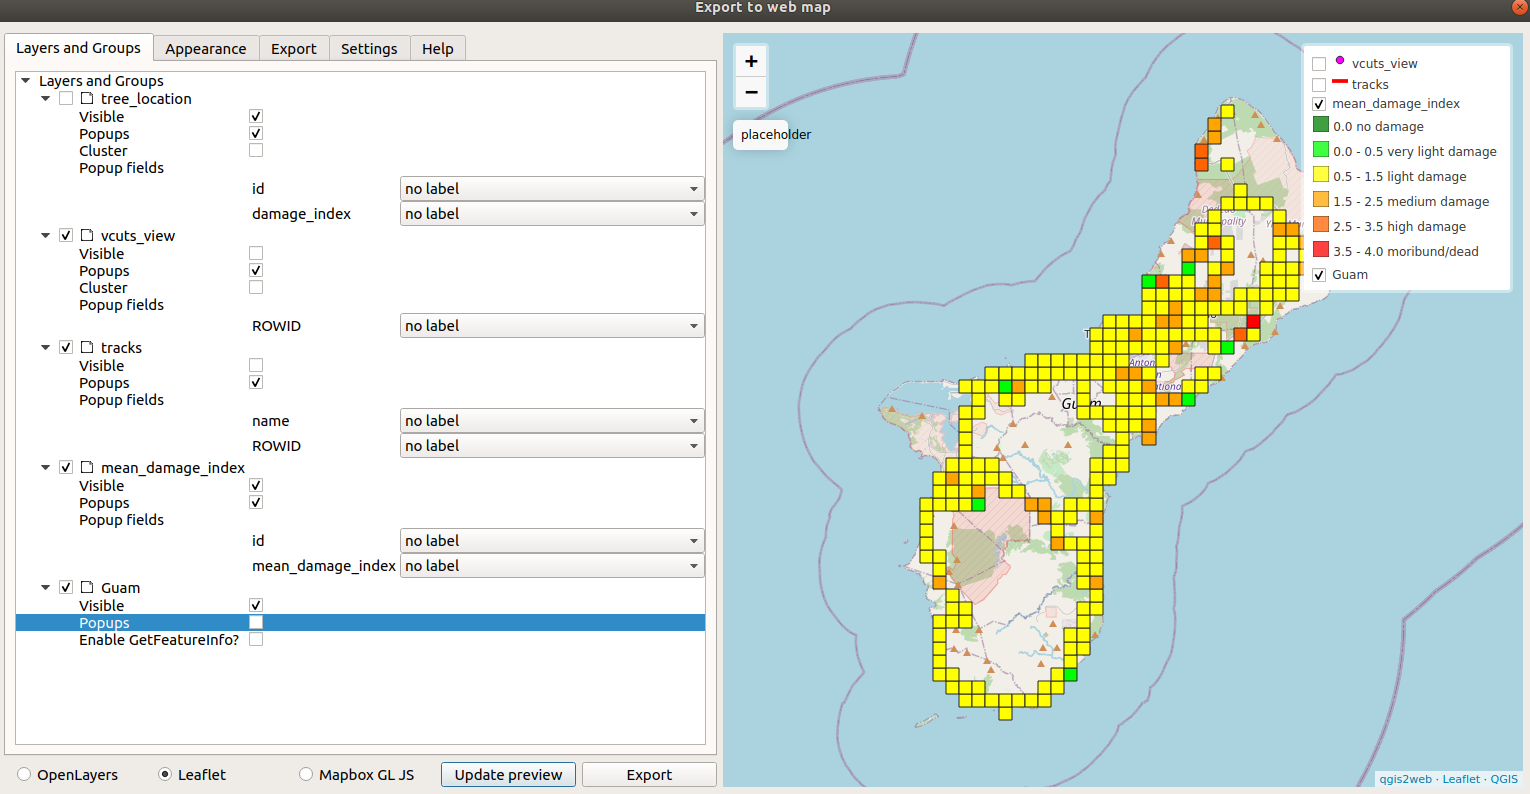
\includegraphics[width=\linewidth]{images/qgis2web1.png}
	\caption{\textbf{qgis2web} parameters Screenshot 1.}
	\label{fig:qgis2web1}
\end{figure}

\begin{figure}[H]
	\centering
	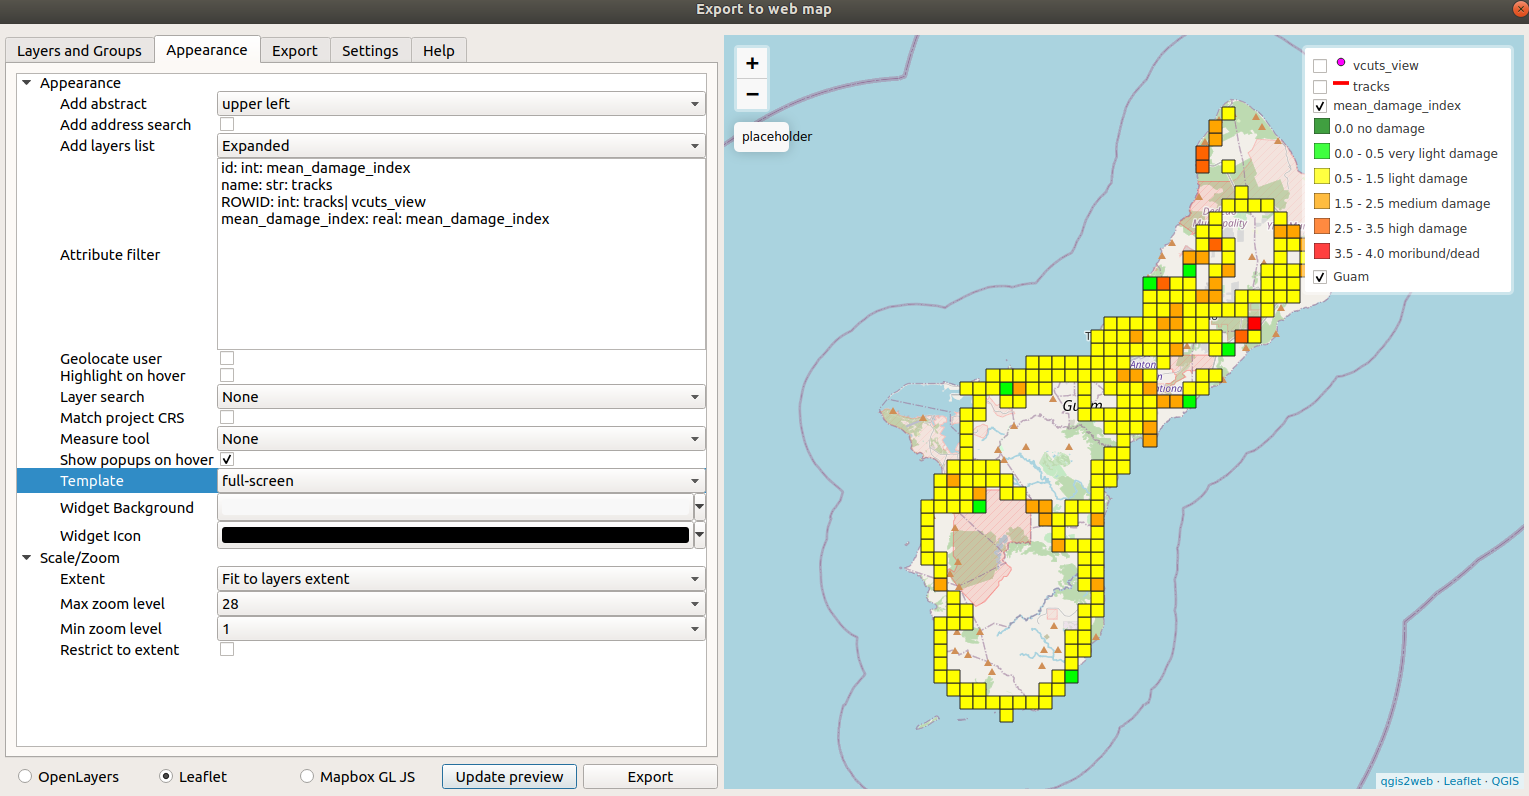
\includegraphics[width=\linewidth]{images/qgis2web2.png}
	\caption{\textbf{qgis2web} parameters. Screenshot 2.}
	\label{fig:qgis2web2}
\end{figure}


\section{First Roadside Video Survey of CRB Damage on Guam}

\subsection{Methods}

\begin{tabular}{|l|l|l|}
	\hline 
	& \textbf{Development} & \textbf{Guam01 survey} \\ 
	\hline 
	Vehicle & Mazda Miata & Toyota Forerunner \\ 
	\hline 
	Cell phone & Samsung Galaxy S10 & Samsung Galaxy S8 \\ 
    \hline 
	Lens & Ultra-wide angle & Standard angle \\
	\hline
	Frame rate & 30 FPS & 15 FPS \\
\hline
\end{tabular} 

\subsection{Results}

Data and results from the Guam01 survey are available in a public GitHub repository \cite{mooreGitHubRepositoryGuamCRBdamagemap2020102020}. An interactive web map is available on GitHub pages (Fig. \ref{fig:guam01webmap}).

\begin{figure}[H]
	\centering
	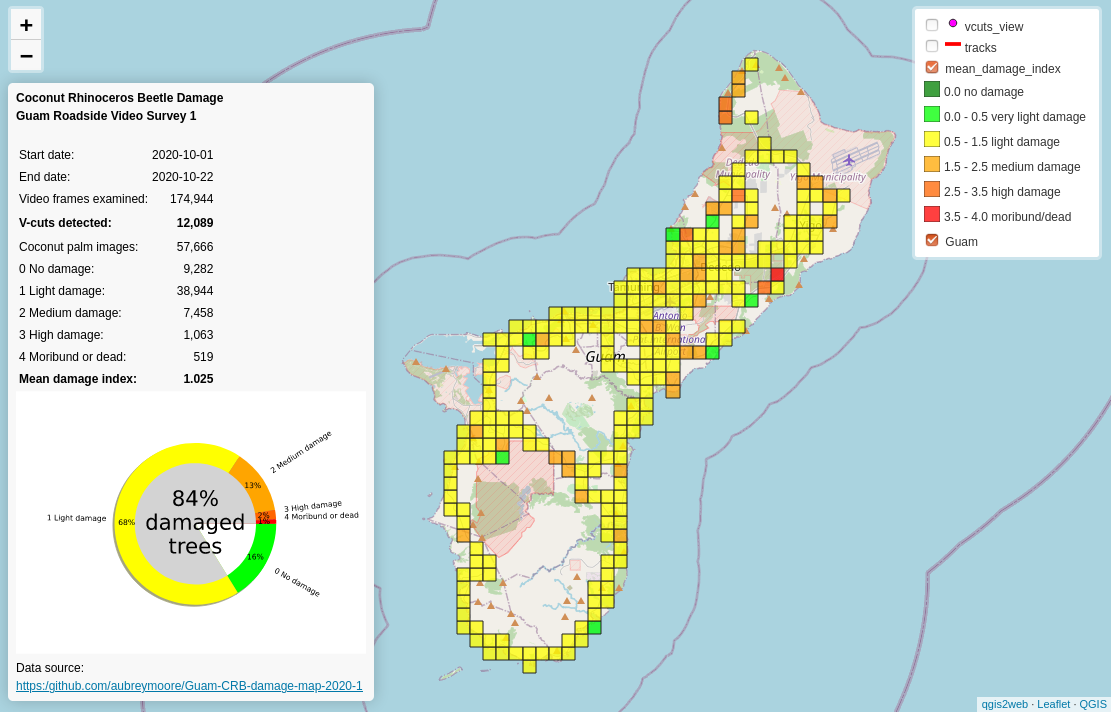
\includegraphics[width=\linewidth]{images/Guam01-webmap}
	\caption{Screenshot of an interactive web map of results from the Guam01 roadside video survey of CRB damage on Guam (\cite{mooreWebMapGuamCRBdamagemap2020102020}) URL: \url{https://aubreymoore.github.io/Guam-CRB-damage-map-2020-10}.}
	\label{fig:guam01webmap}
\end{figure}


\section{Extra}

\cite{aubreymooreSetAutomatedRoadside2020}

\cite{onepanelinc.AIPipelineOperations2020}

\cite{onepanelinc.ScopeWorkObject2020}

\newpage
\section{Test Data}

The following creates a 30 second video clip starting at 10 minutes and 30 seconds after the start of the video.
Start time = 10:46:54 + 00:10:30 = 10:57:24.

\begin{verbatim}
mv 20210304_104654.mp4 20210304_104654_original.mp4
ffmpeg \
    -ss 00:10:30 \
    -i 20210304_104654_original.mp4 \
    -ss 00:00:30 \
    -t 00:00:30 \
    -c copy \
    20210304_104654.mp4
\end{verbatim}

Unfortunately, timestamps in the resulting file are not set, so we have to edit using:

\begin{verbatim}
exiftool "-CreateDate=2021:03:04 10:57:24" 20210304_101635.mp4
\end{verbatim}


\printbibliography	

\end{document}
